\chapter{Daemons}
\label{app:B}

An important component PREGO approach (Figure A1) is the regular updates which keep PREGO in line with the literature and microbiology data advances. The updates are implemented with custom scripts called daemons that are executed regularly spanning from once a month up to six-month cycles. This variation occurs because of the API requirements of each web resource as well as the computational intensity of the association extraction from the retrieved data.

\begin{figure}[h]
   \centering
   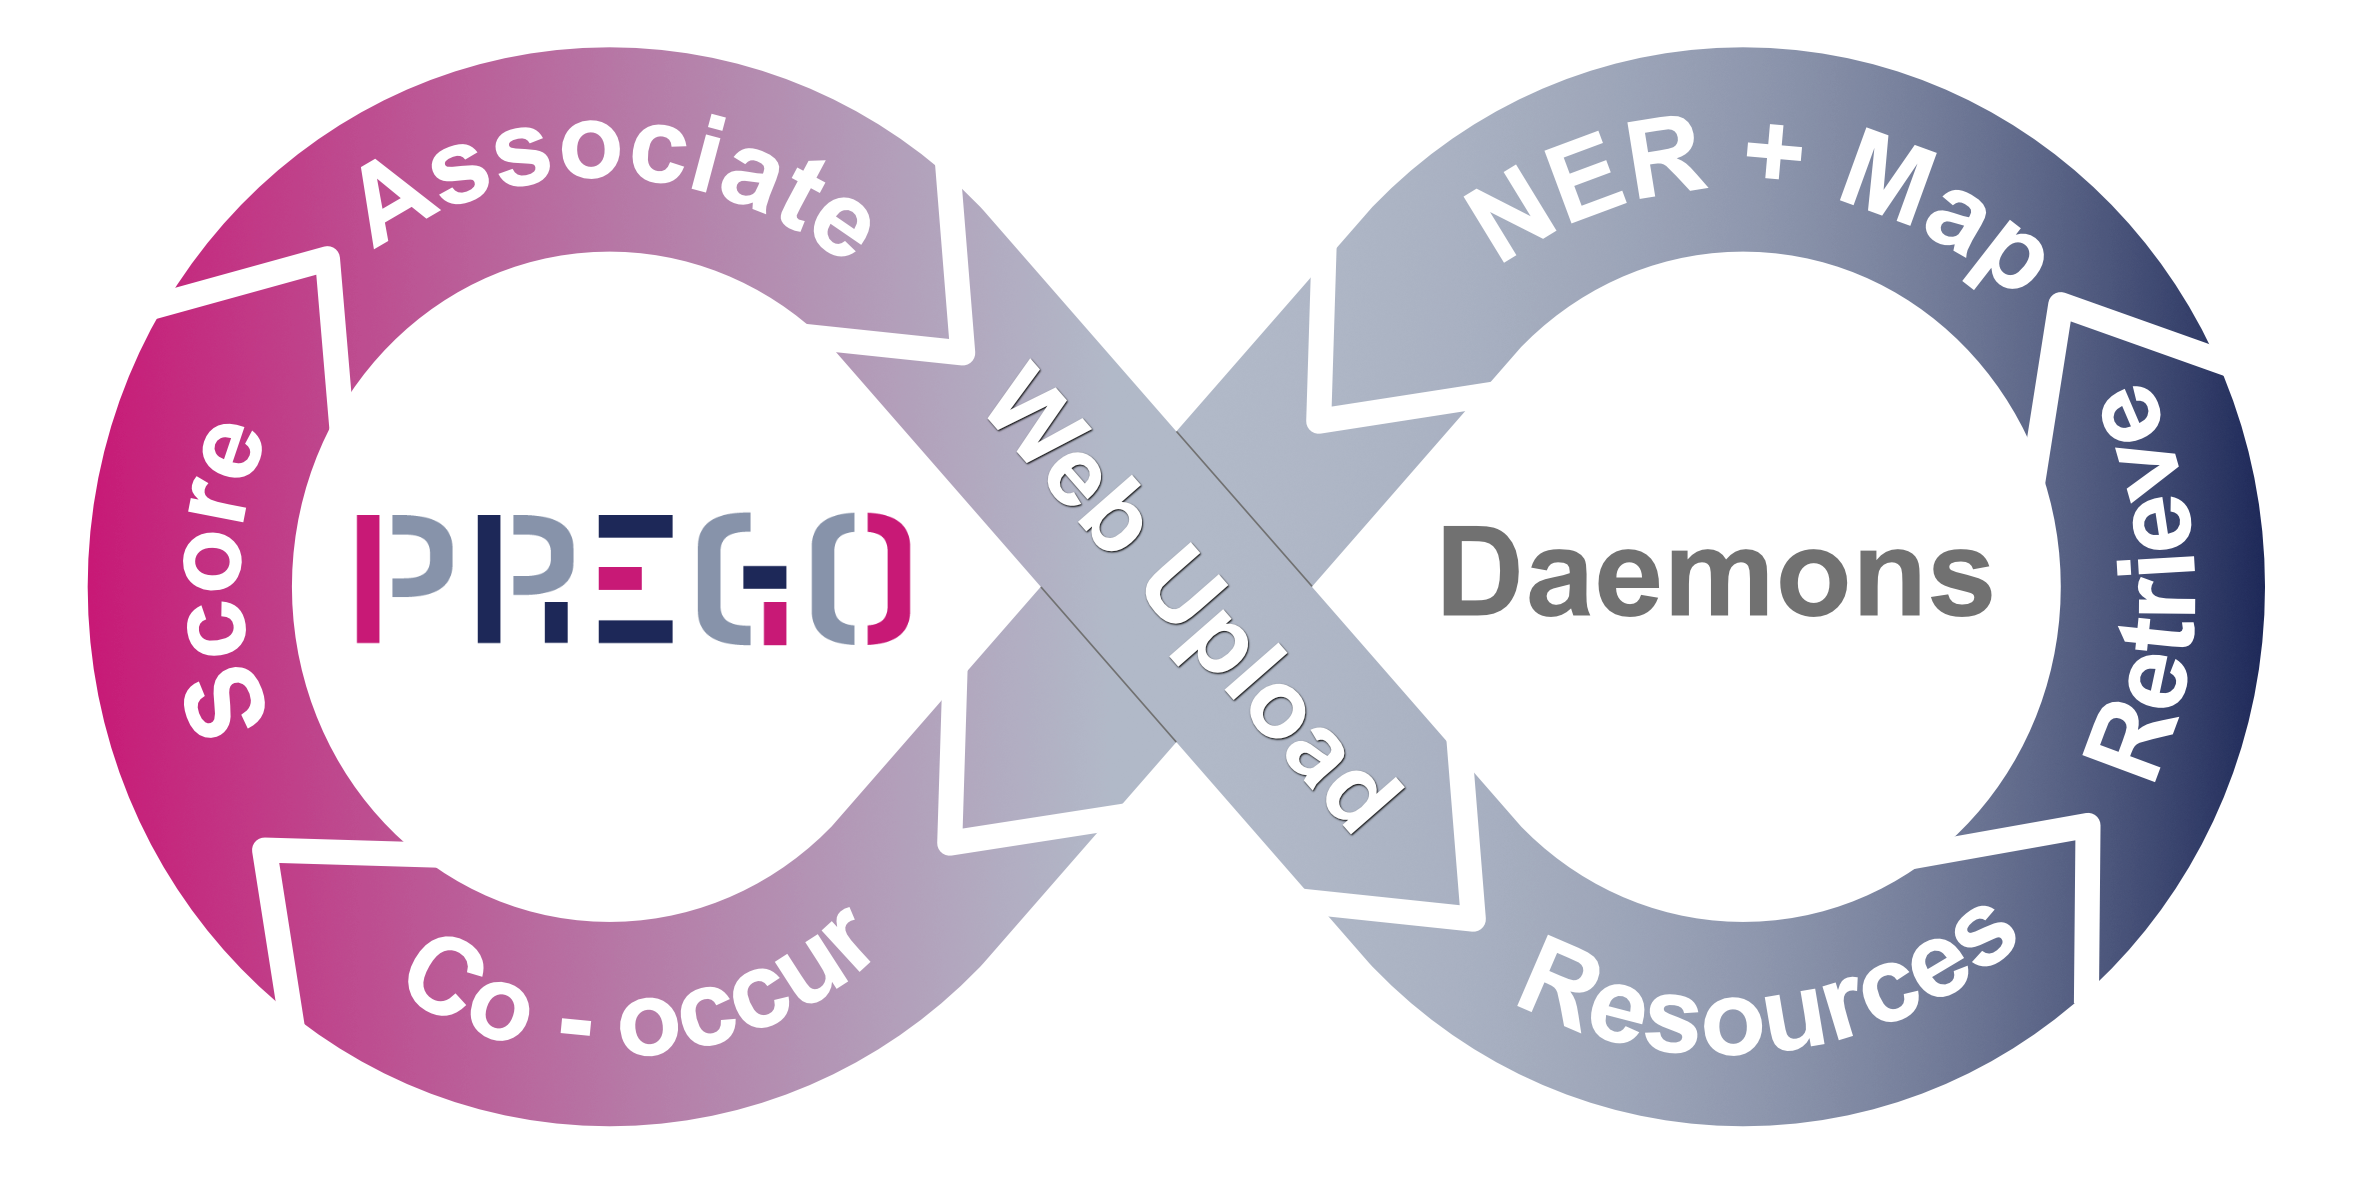
\includegraphics[width=95mm]{figures/figure_A1_PREGO_daemons.png}
   \caption[PREGO DevOps]{Software daemons perform all steps of the PREGO methodology in a continuous manner similar to the Continuous Development and Continuous Integration method.}
   \label{fig:devops}
\end{figure}


Each Daemon is attached to a resource because its data retrieval methods (API, FTP) and following steps, shown in Figure A1, require special handling and multiple scripts (see \textit{prego\_daemons} in the Availability of Supporting Source Codes section).